\chapter{Data Flow}

[todo]
Block Diagram
- With different stages.
- And Explain Data Inputs and Data Outputs of each stage. 

The end to end system consist of four main stages viz., image sensor, image signal processor(ISP), processor, and Off-chip memory. The image sensor captures raw images, which are processed by ISP to generate RGB images, which are used by processor/accelerator, and the DRAM supports for storage of images and data for all the above stages. The ISP is typically integrated with the processor SoC, and Camera and DRAM are implemented in separate chips. 

\section{Monoscopic 360 }
\begin{figure}[h]
	\begin{center}
		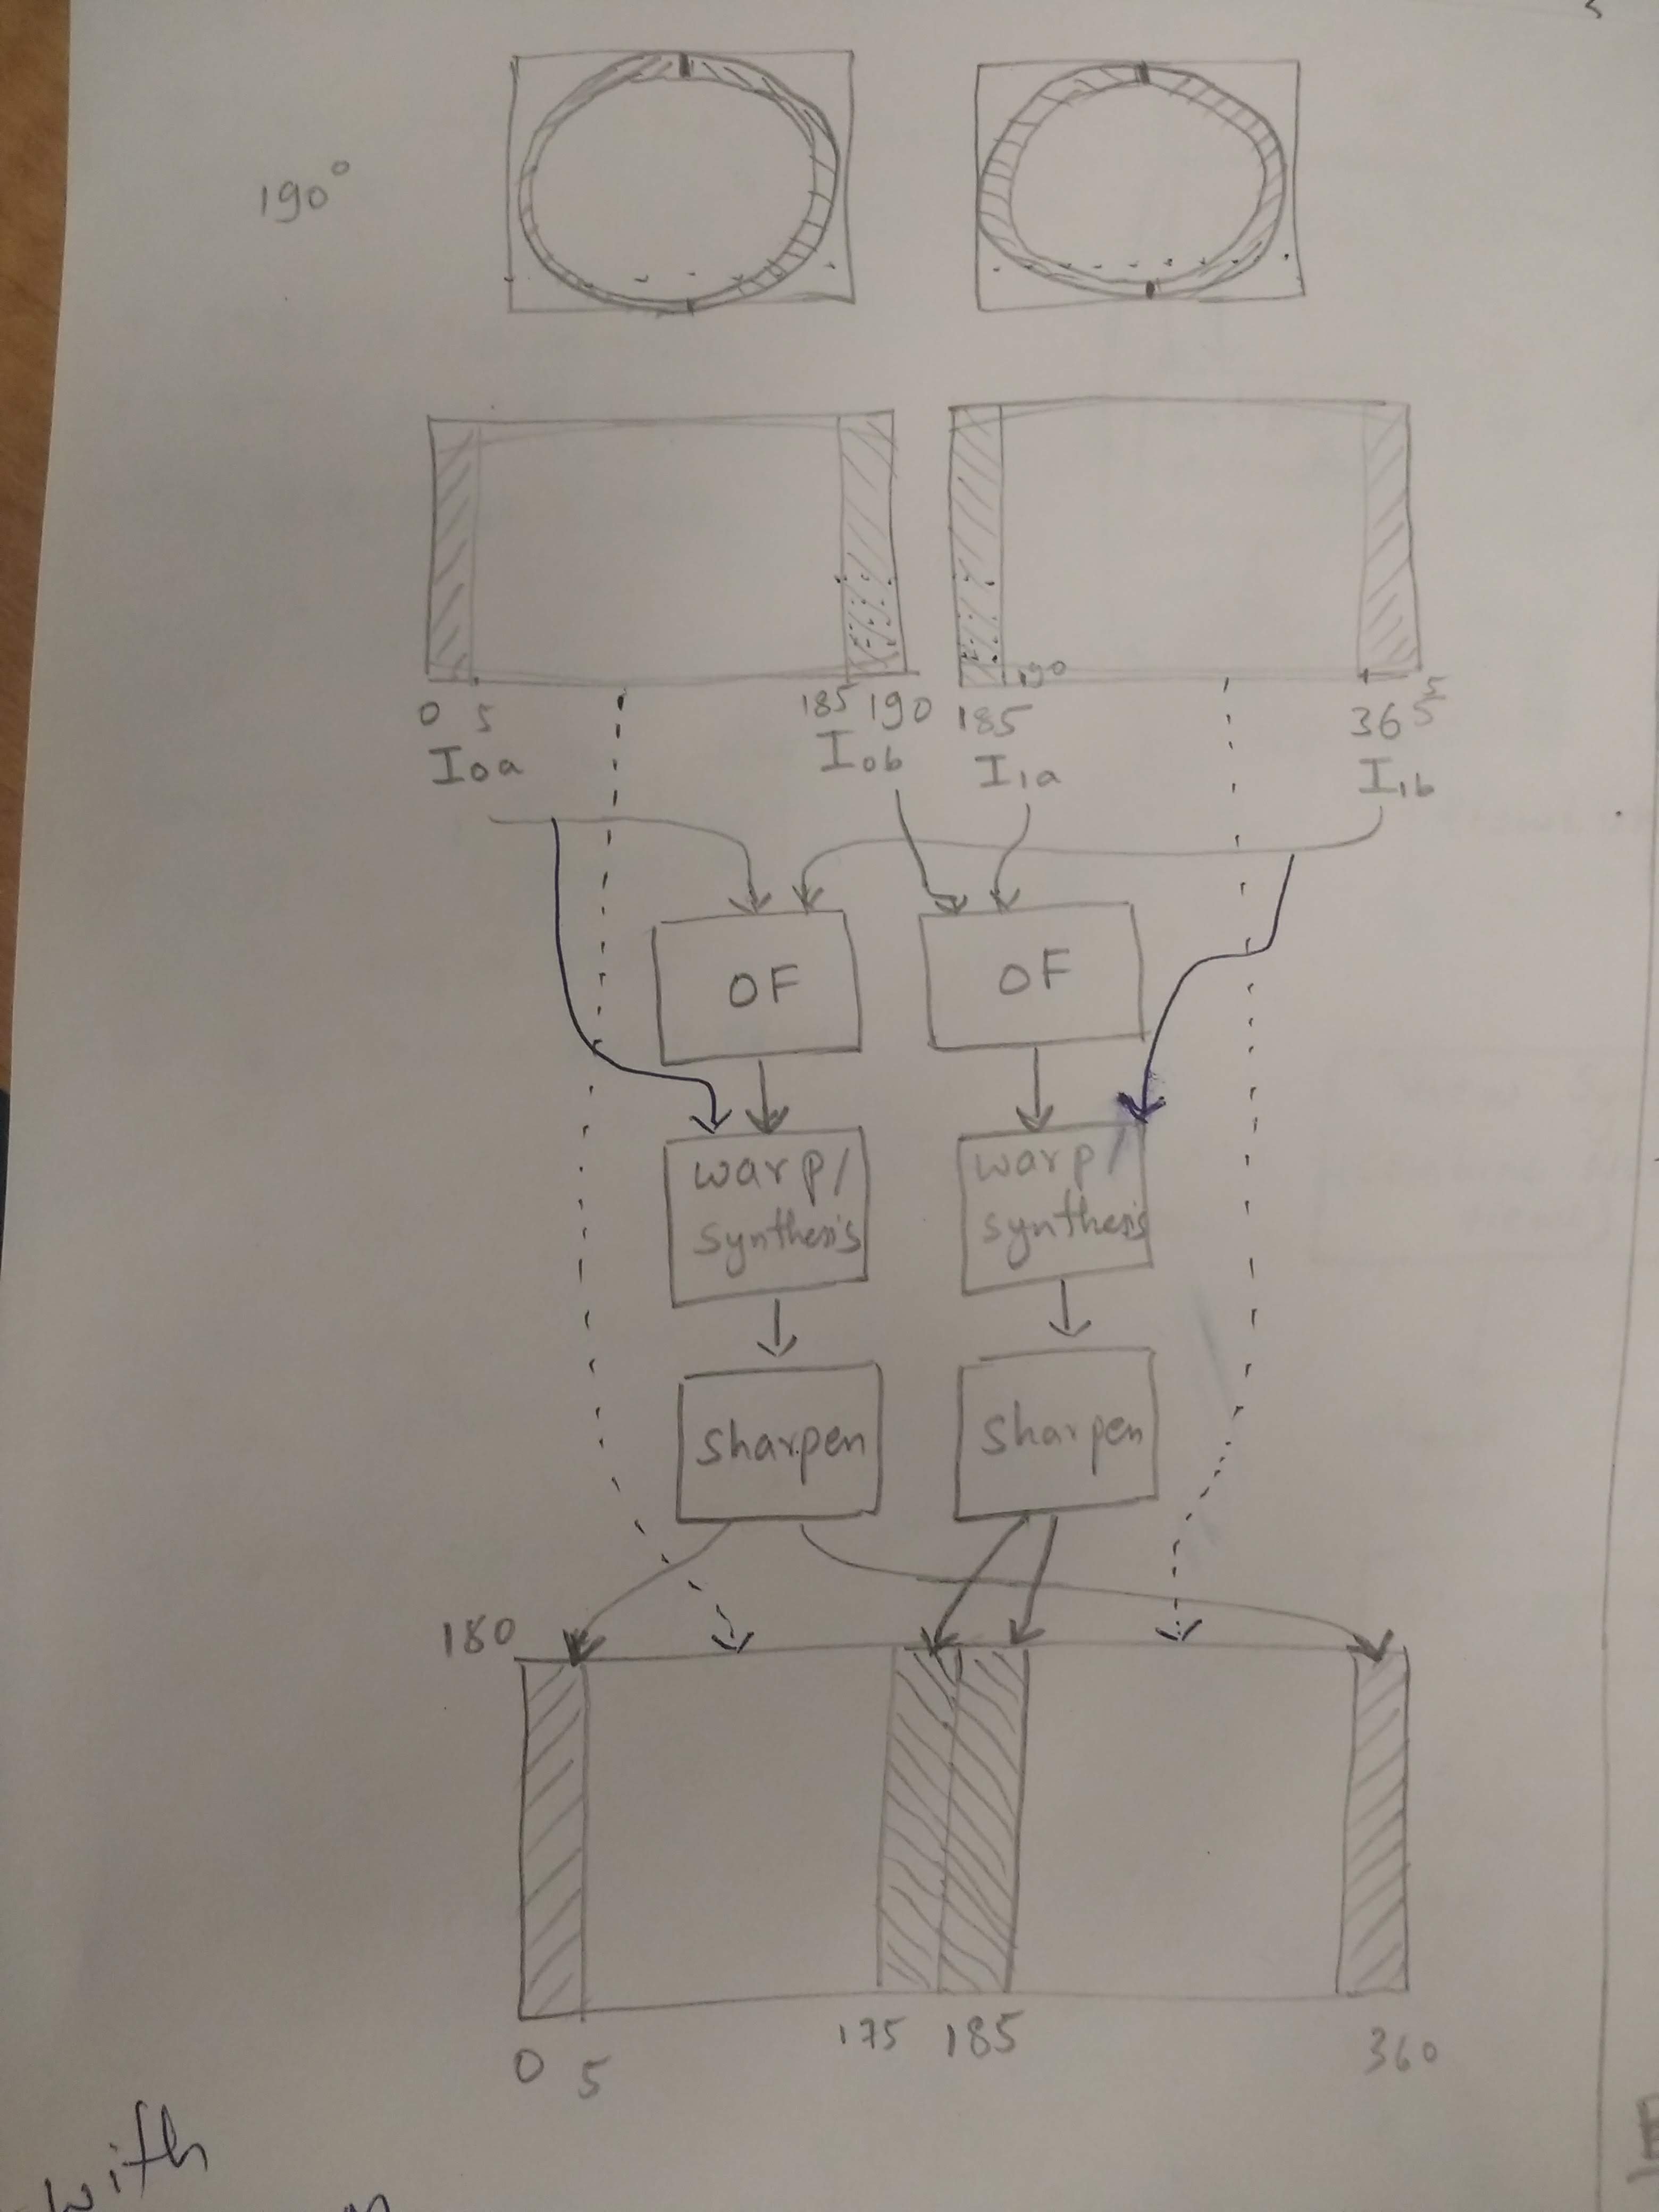
\includegraphics[width=0.5\textwidth]{/media/gunman/Data/thesis/ThesisLatex/data/images/Monoscopic_input_output.jpg}
		\caption{Data-flow block diagram dipicting different stages and their inputs and outputs in the end-to-end pipeline in monoscopic 360}
		\label{Monoscopic_Input_Output}
	\end{center}
	\vspace{-0.3in}
\end{figure} 


Fisheye lenses allow image sensors to capture images within an ultra-wide hemispheric field of view. With two fisheye-lensed sensors that capture complementary fields of view each of over 180 \textdegree  , the pair of captured images can be processed to achieve over a spherical 360 \textdegree  x 180 \textdegree   area, as shown in Figure 2. The equirectangular projection format is a common format for 360 \textdegree  x180 \textdegree   images, allowing remapping to other projections for convenient viewing. To create equirectangular images, the paired fisheye capture data undergoes multiple stages:
1) Projection Mapping: The equirectangular image is populated by sourcing image pixels from the fisheye images along a (spherical coordinate → polar coordinate) projection map. As projected pixel coordinates typically fall between integer pixel coordinates, the algorithm typically either pulls a nearest-neighbor pixel or a bilinear combination of a neighborhood of pixels. 
2) Correspondence:  As the two fisheye cameras do not precisely occupy the same point in space, objects at the edges of fisheye images appear in different positions in the images, dependent on their distances from the camera. This phenomenon is called the parallax effect. To ensure that objects appear properly, a correspondence algorithm identifies matching visual features across image pairs, warping the projection to reduce object seams in the image.
3) Blending: Even after projection and correspondence suggest image overlay coordinates, intensity variations from misalignments still occur between the two projected images at the stitching boundary. The blending stage combines the images through a weighted sum of pixel values to generate a seamless 360 \text degree   image with a smooth transition.	
4) Compression: To reduce the bandwidth at the capture, networking, or storage interface, images can be compressed into representations that use smaller file sizes. Lossy compression schemes, e.g., JPEG/MPEG, allow dramatic reductions in file size by discarding information that is considered to be perceptibly irrelevant.
\subsubsection{Hardware}
Hardware: Dual Fisheye Camera \newline
Monoscopic Stages:
The stages may include Intensity compensation, fisheye unwarping, alignment, blending. 
\begin{figure}[h]
	\begin{center}
		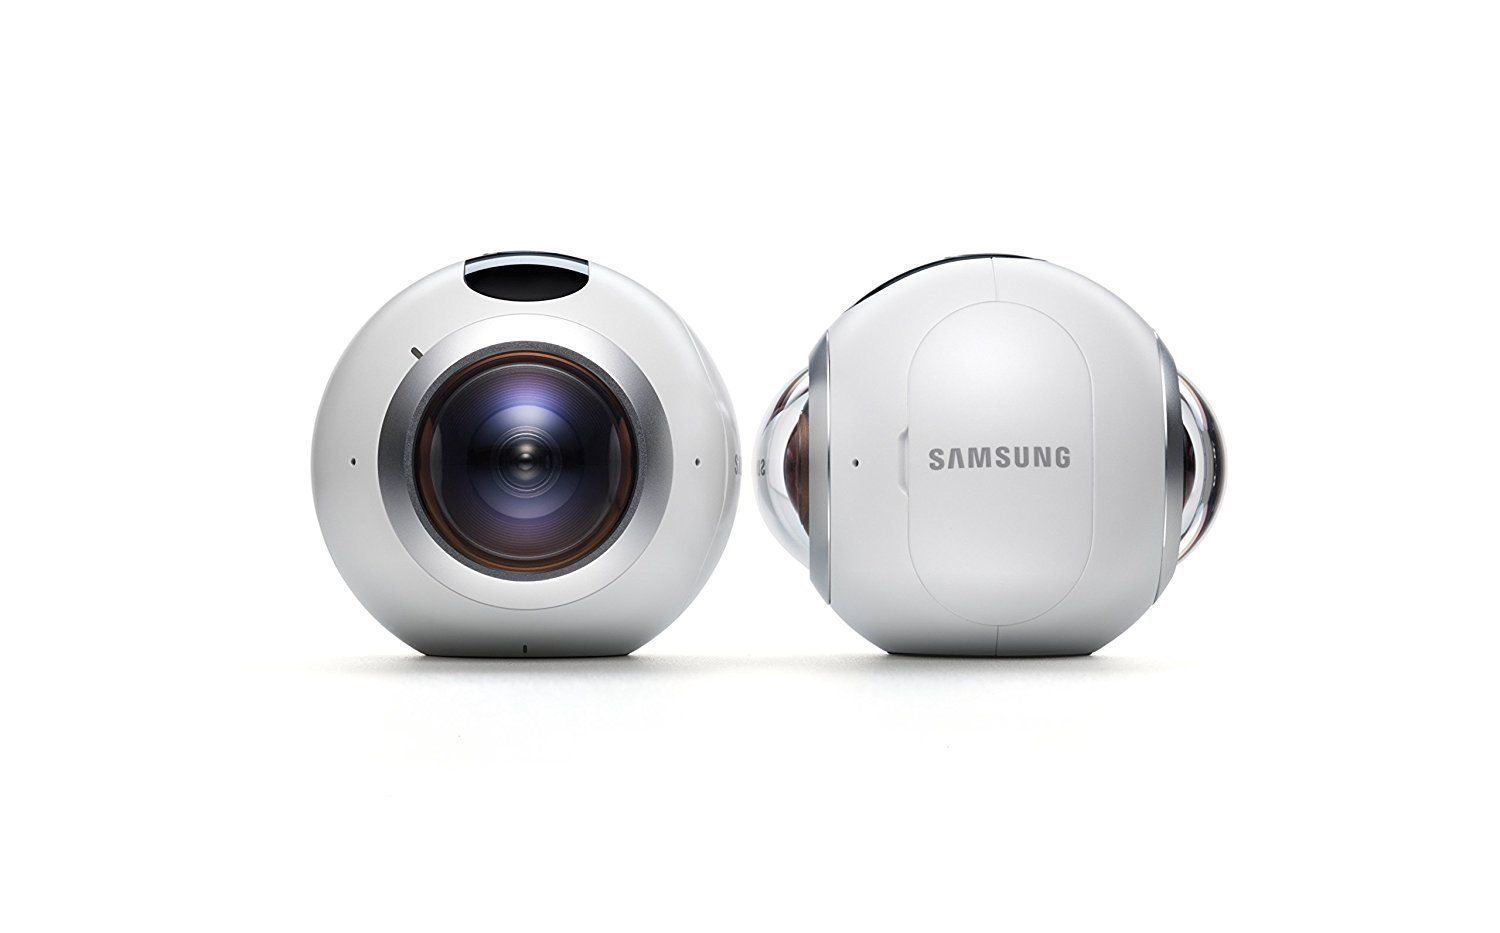
\includegraphics[width=0.6\textwidth]{/media/gunman/Data/thesis/ThesisLatex/data/images/Samsung-Gear-360-Real-360.JPG}
		\caption{Dual fisheye gear 360 device used for capturing monoscopic video}
		\label{ODS_Input_Output}
	\end{center}
	\vspace{-0.3in}
\end{figure} 





\section{Omni-directional Stereo System}
\begin{figure}[h]
	\begin{center}
		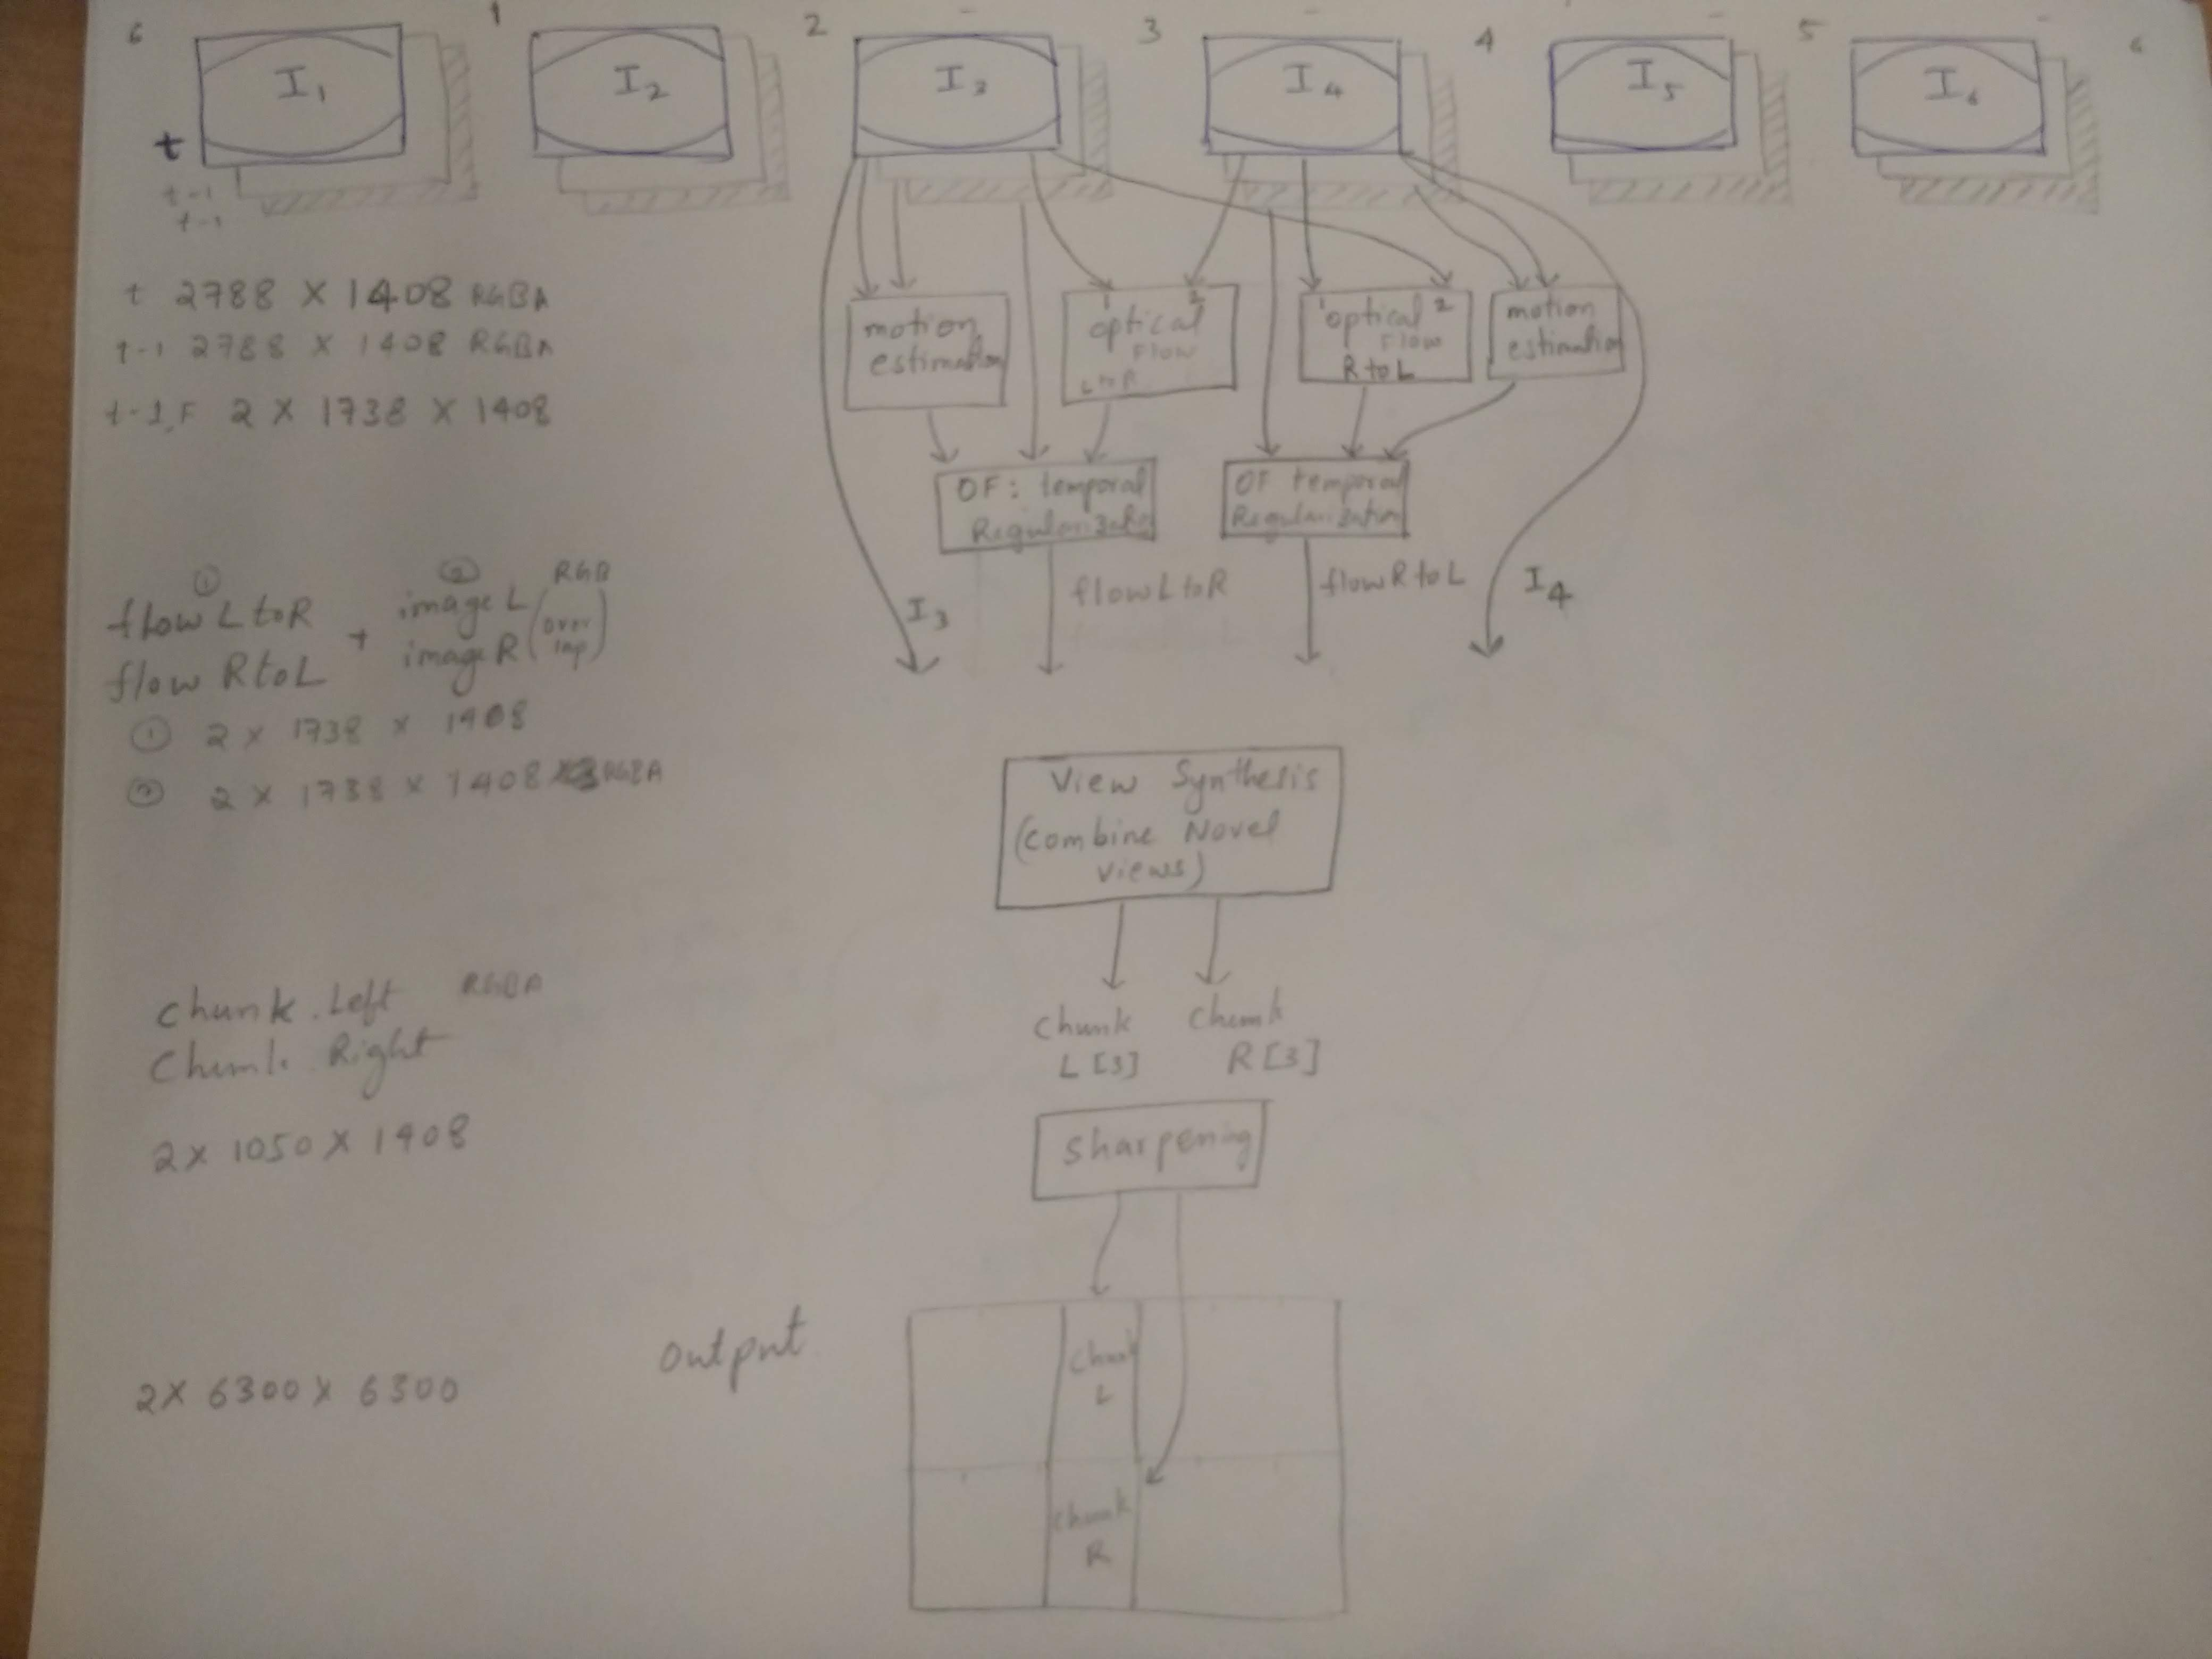
\includegraphics[width=1\textwidth]{/media/gunman/Data/thesis/ThesisLatex/data/images/ODS_Input_Output.jpg}
		\caption{Data-flow block diagram dipicting different stages and their inputs and outputs in the end-to-end pipeline in ODS}
		\label{ODS_Input_Output}
	\end{center}
	\vspace{-0.3in}
\end{figure} 

\begin{figure*}
	\begin{center}
		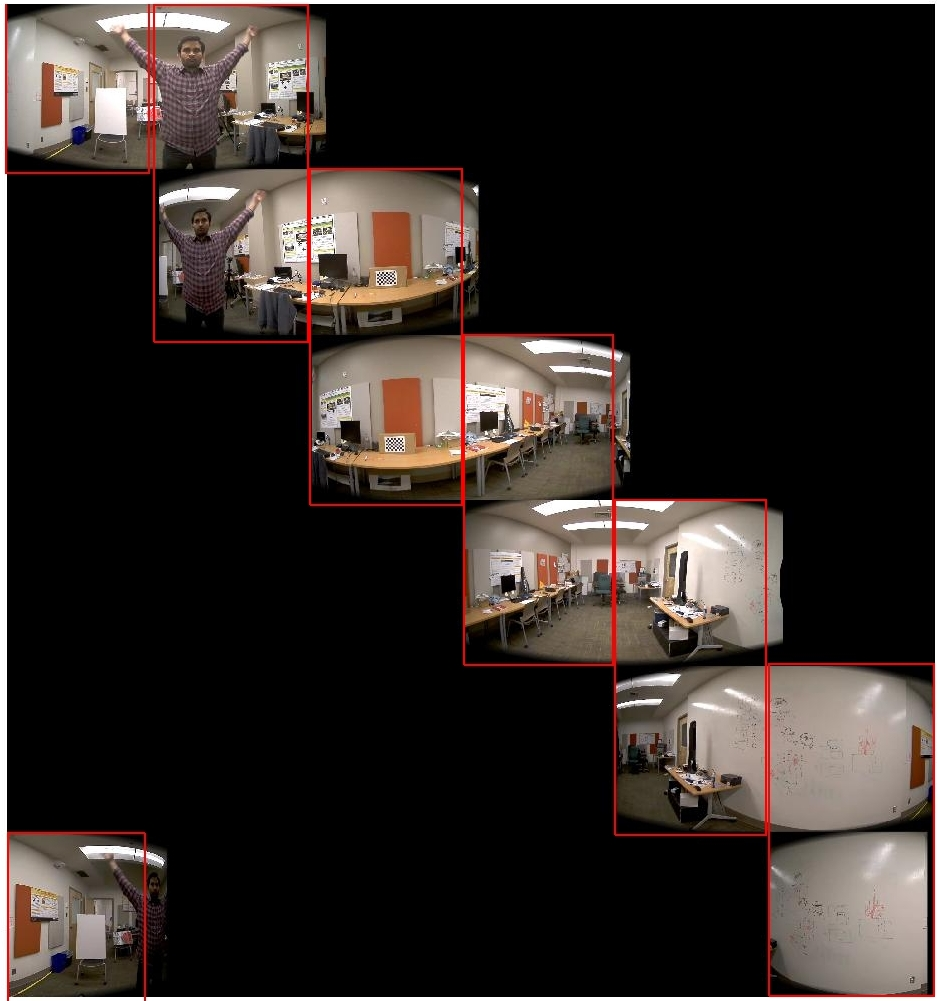
\includegraphics[width=0.8\textwidth]{/media/gunman/Data/thesis/ThesisLatex/data/images/EqRect_offset_fov_viz_loop v3.jpg}
		%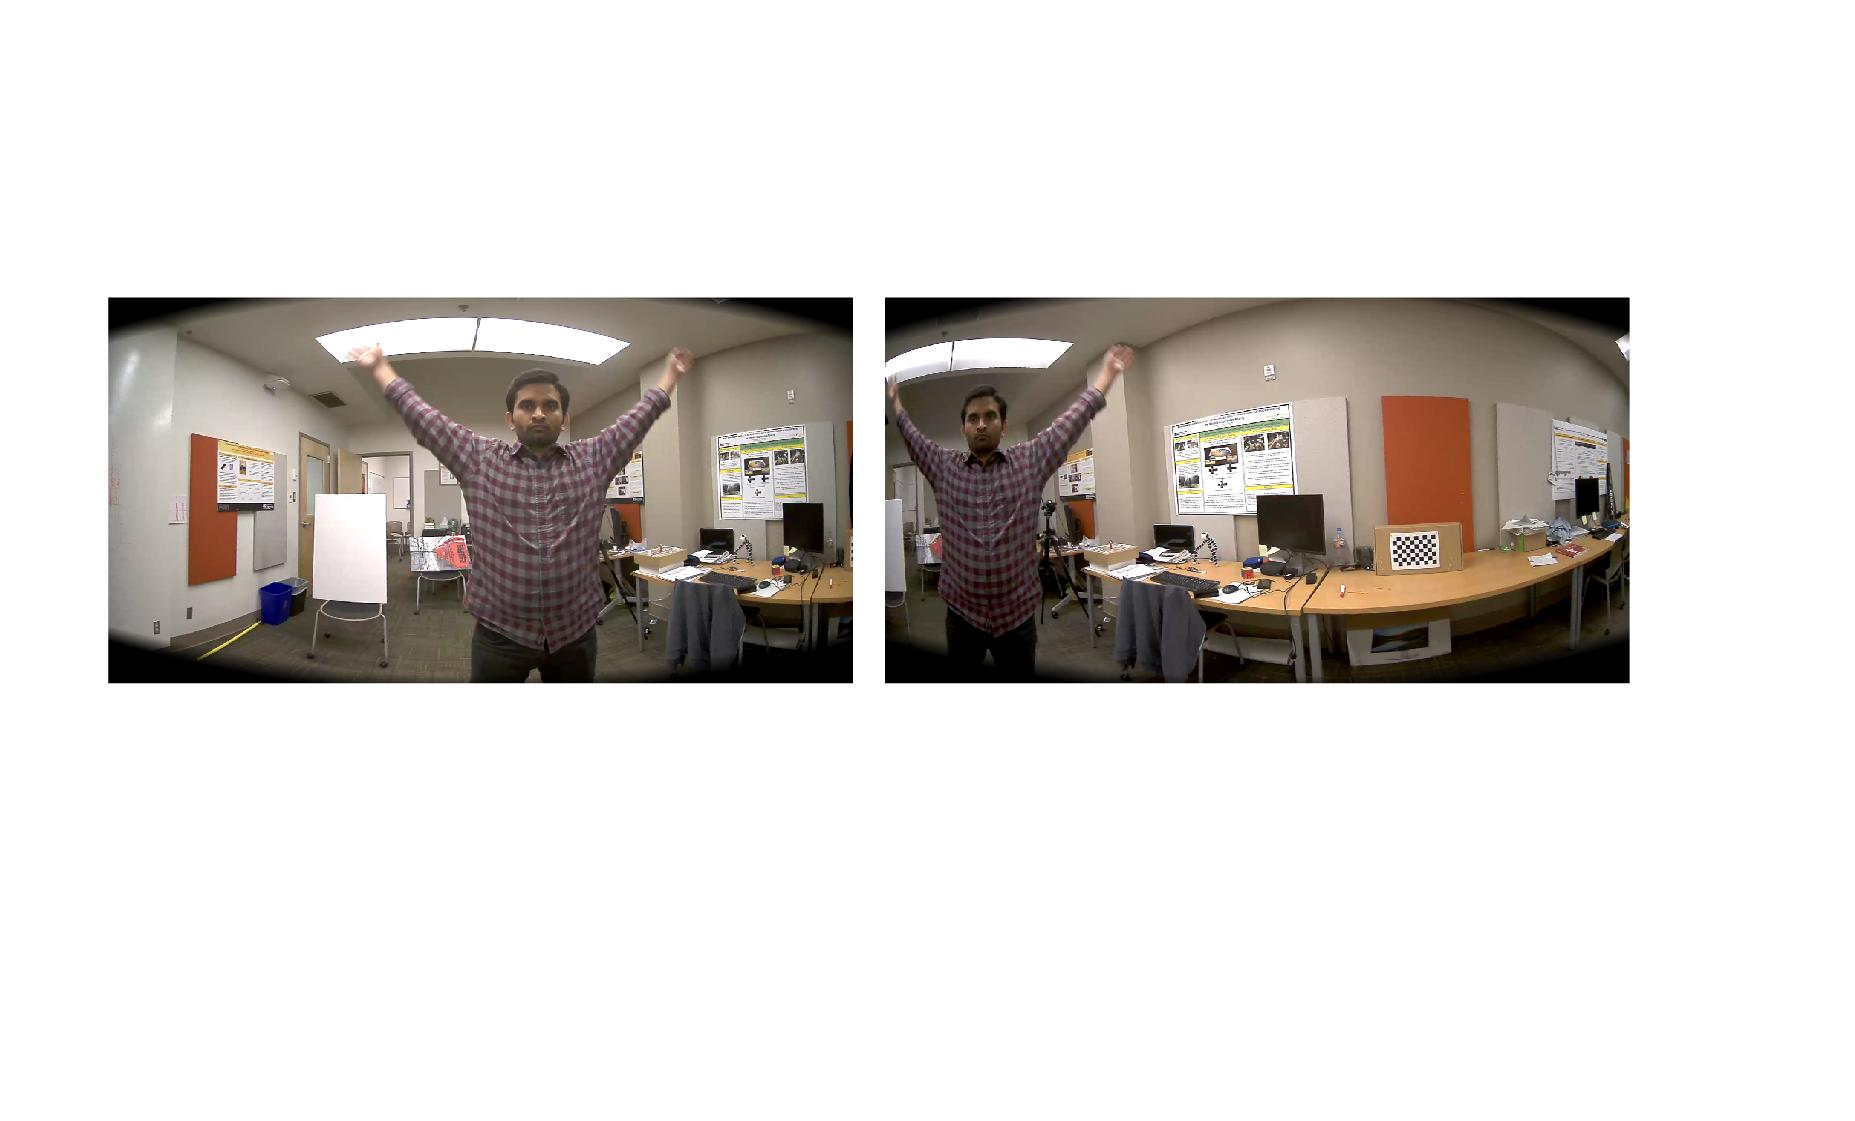
\includegraphics[width=1.1\textwidth]{/media/gunman/Data/thesis/ThesisLatex/data/images/EqRect_2_adj_images.jpg}
		\caption{Equirectangular Projection of first and second camera frames}
		\label{ODS_Input_Ouput}
	\end{center}
	\vspace{-0.3in}
\end{figure*} 

The overlapping left and right images.
\begin{figure*}
	\begin{center}
		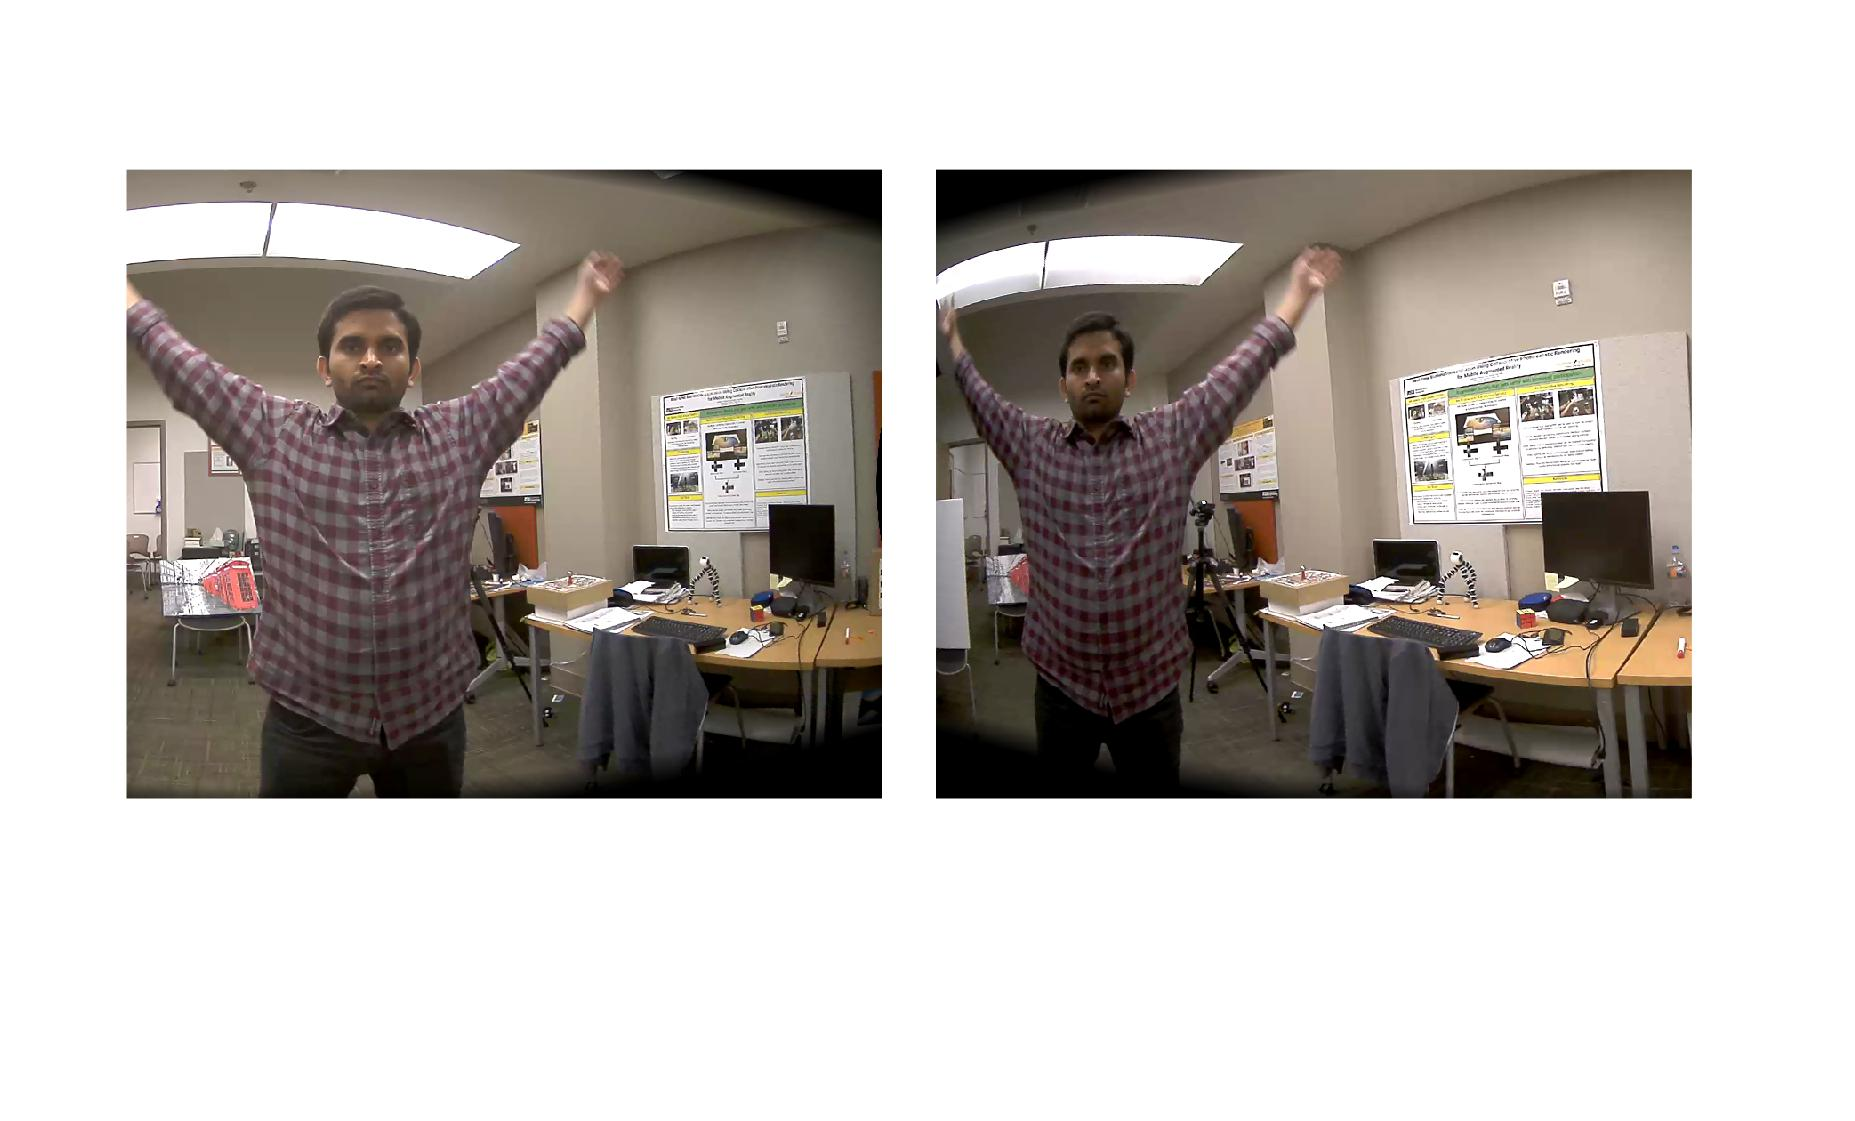
\includegraphics[width=1.1\textwidth]{/media/gunman/Data/thesis/ThesisLatex/data/images/OF_inp_overlap_region_of_adj_cam.jpg}
		\caption{Optical flow inputs: Overlapping regions of adjacent camera images. Equirectangular Projection of first and second camera frames}
		\label{ODS_Input_Ouput}
	\end{center}
	\vspace{-0.3in}
\end{figure*} 

Hardware:Six Camera Rig.
For our prototype camera design we use six IMX-274 cameras for capture and Nvidia Jetson TX2 for stitching. The Camera and Jetson specs are shown in figure 3.2. \newline 
\begin{figure}[h]
	\begin{center}
		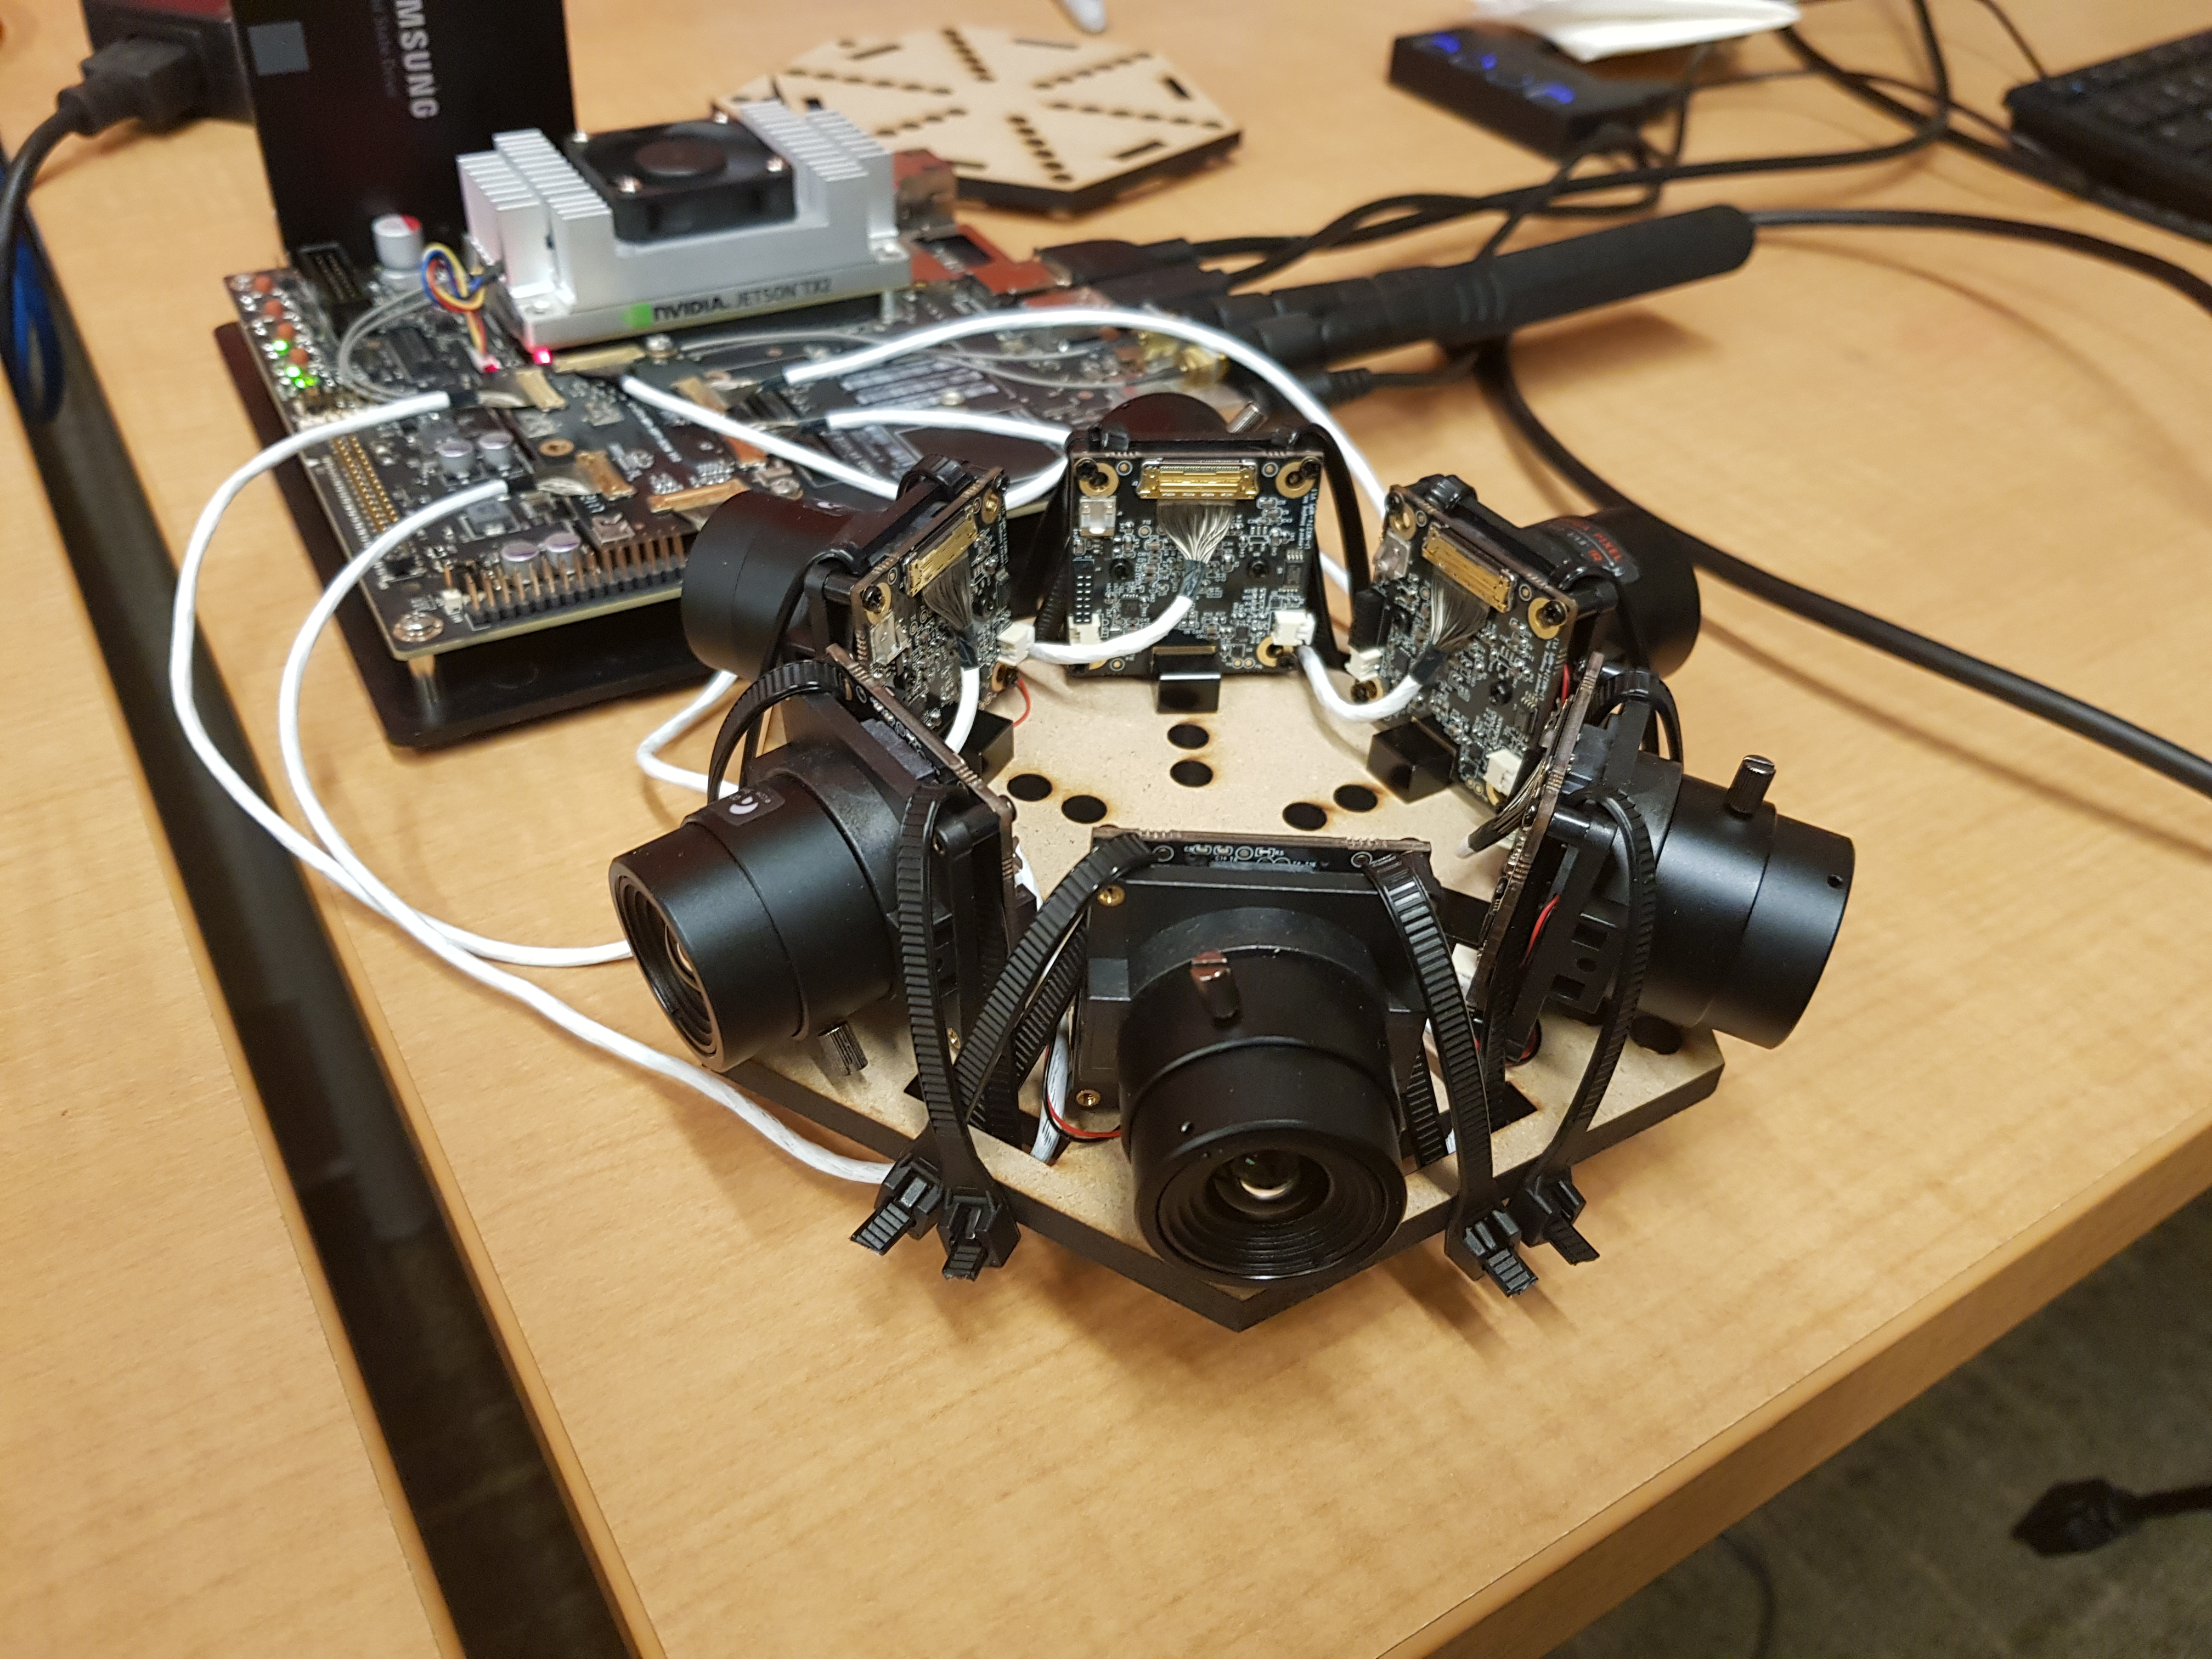
\includegraphics[width=0.5\textwidth]{/media/gunman/Data/thesis/ThesisLatex/data/images/six_camera_rig.jpg}
		\caption{ODS Camera Rig}
		\label{ODS_Input_Output}
	\end{center}
	\vspace{-0.3in}
\end{figure} 

\begin{tabular}{c|c}
	Camera Name & Sony IMx274 \\
	Output Image Size & Diagonal 7.20 mm (Type 1 / 2.5) aspect ratio 16:9 \\
	Number of Effective Pixels & 3864 (H) x 2202 (V) approx. 8.51M pixels \\
	Unit cell size & 1.62 um (H) x 1.62 um (V) \\
\end{tabular} \newline

Software:
Nvidia libargus Camera API,
openCV, C++ \newline

Data Flow Diagram
- With different stages

The main goal of this work is to reduce bandwidth requirement and remove redundant computation during different stages. 



\section{Challenges with existing systems}

\begin{figure}[h]
	\begin{center}
		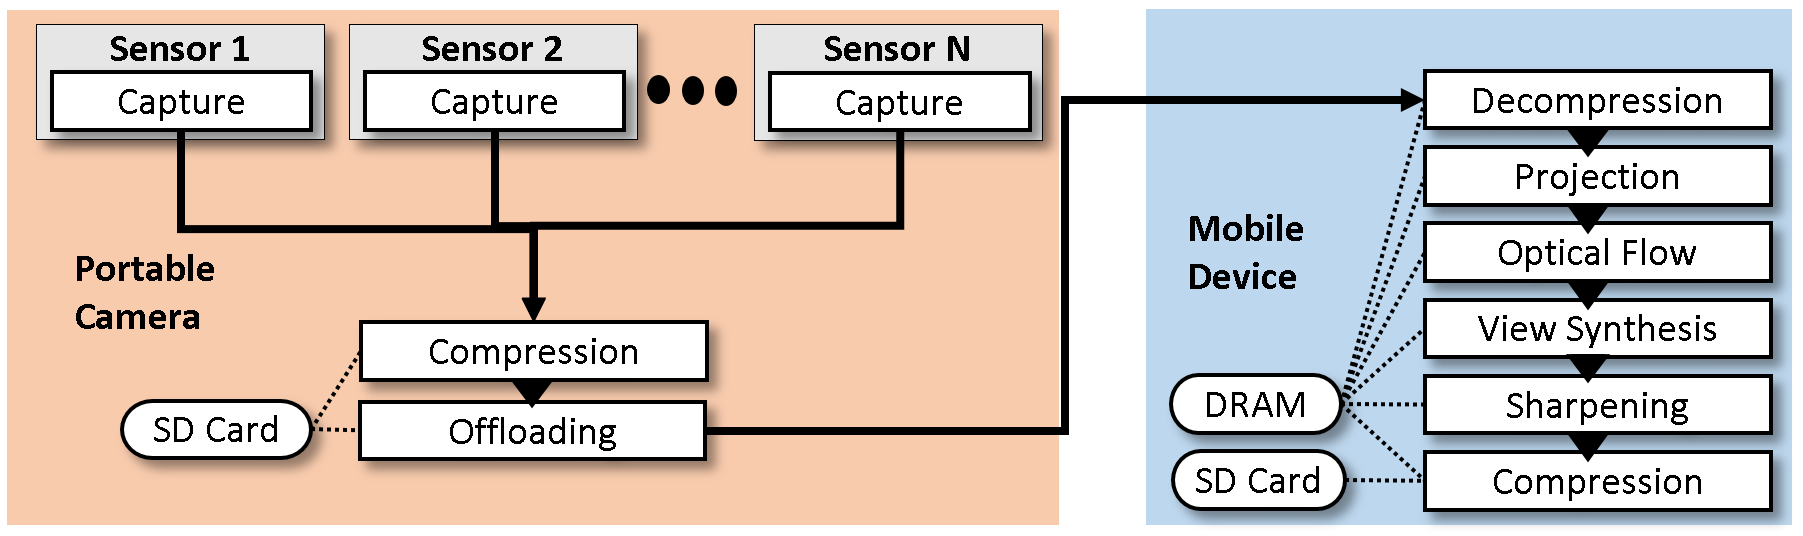
\includegraphics[width=1\textwidth]{/media/gunman/Data/thesis/ThesisLatex/data/images/Offline_stitching_Arch.PNG}
		\caption{General Off-loading based system pipeline}
		\label{fig:ex_4_9}
	\end{center}
	\vspace{-0.3in}
\end{figure} 

\subsection{Energy}
Data and power numbers for Google Jump VR:
Number of cameras: 17
Data Generated per each frame by 17 cameras(in bayer): 816 MB

Data bandwidth requirement in Gb/s : 47.8 Gb/s
(@30fps, compressed data(1:8 compression ratio))

Power:
Camera Capture and basic processing at camera:  50 W
DRAM power(approx.) : 61 W 
(30 W corresponds to store data generated by 30 frames of all 17 cameras)
On chip LVDS power(approx): 19 W
(For transferring one frame of all 17 cameras)
Compute Power: ( very high, done offline using multiple GPU's)
Facebook also has 360 stereo solutions, one with 24 cameras and other with 6 cameras. I may need to find data for them as well. Consumes similar amount of power.
\subsection{Latency}
Several hours for final ODS generation.
